\chapter{Trustless Timestamping}
\label{chpr:trustless}
Bitcoin enables timestamping in a trustless framework. 
To show this first we introduce what Bitcoin is and why it works, then we show two techniques to timestamp data using the protocol's digital coins.

As a premise it is important to highlight why and in which terms a trustless design is superior to a trusted one. 
Trusted schemes can be built upon trustless ones, but the other way around is not possible. 
Trustless systems have higher security but the mechanism sustaining it makes thing much more sophisticated, yielding to less accuracy and efficiency with respect to trusted ones.

\section{Bitcoin}
\label{bitcoin}
Bitcoin is an electronic payment system based on cryptography rather than trust. A \textit{coin} is defined as a chain of digital signatures. Each owner transfers the electronic coin to the next by digitally signing a hash of the previous \textit{transaction} and the public key of next owner (or a commitment to it).

Coins doesn't have to be managed individually, they can be combined and split in transactions containing multiple inputs and outputs. The last output appended to a coin is said unspent transaction output, UTXO.

However who receives a transaction cannot verify that who pays him did not \textit{double-spend} the coin. 
To prevent this behaviour it is needed a system to agree on a single history of the order in which the transactions were received. The proposed solution starts with a timestamp server: each timestamp it's a hash of a \textit{block} which contains a set of items and the previous timestamp (if there is one). The resulting data structure forms a chain, which is often referred to as \textit{blockchain}\footnote{In \cite{Nakamoto_bitcoin:a} it is referred as block chain, later the term blockchain became used regularly. However, as of writing, such term is associated with an excessive hype which is misguiding the technological development.}. 
\begin{equation}
	TS_i =
	\begin{cases} 
		h(items_0) & i=0\\ 
		h(TS_{i-1} || items_i) & i=1, ..., i_{max} 
	\end{cases}
\end{equation}
To implement a \textit{distributed} version of a timestamp server it is used a \textit{proof-of-work} (PoW) system similar to Adam Back's Hashcash \cite{Back02hashcash-}. The proof-of-work consists in scanning for a value (called \textit{nonce}) to be included in the block that when hashed produces an hash value (interpreted as an integer) less then a given target $w$ as pointed in Definition \ref{pow}.

\begin{mydef}The {\textit{proof-of-work}} consists in:
\label{pow}
\\
\textbf{given}:
\begin{itemize}
	\item previous timestamp $TS_{i-1} \in \{0,1\}^n$;
	\item items to timestamp $items_i \in \{0,1\}^*$;
	\item target to beat $w>0$;
\end{itemize}
\textbf{find}:
\begin{itemize}
	\item $nonce \in \{0,1\}^*$ s.t. $h(TS_i || items_{i+1} || nonce) < w$.
\end{itemize}
\end{mydef}

The proof-of-work is basically finding partial hash collisions for the leading zero bits. Hash functions such SHA256 are designed in a way that the fastest algorithm for computing partial collisions is brute force\footnote{Some optimizations have been discovered \cite{DBLP:journals/corr/Hanke16}, but they still require a massive brute force component.}. Thus finding a solution to the challenge is computationally expensive, in other words finding a solution proves that CPU time was consumed and energy was expended for that purpose.
 
If the hash function has a sufficiently large codomain, it can be, in practice, arbitrarily hard to find a solution. For instance consider SHA256, the codomain is $\{0,1\}^{256} \approx \mathbb{Z}_{2^{256}}$, assuming that its outputs have the same probabilities, the chance that a given $nonce$ has hash value less then the target is $\frac{w}{2^{256}}$.  
If $w=1$ the proof-of-work is finding a pre-image of 0 (with additional constraints) but that is not feasible thanks to its preimage resistance property. 
So the lower is $w$ the higher is the difficulty, tending towards an unfeasible problem as $w$ is closer to 1. 
Assuming that the computational power used is known, the target can be chosen so that expected time to find a solution matches a given value.

The proof-of-work is \textit{publicly auditable}: when a solution is found verifiers check its correctness computing a single hash and perform one comparison. If the verification is successful they are convinced that someone has done the work, without the need to know or trust him. In other words \textit{proof-of-work commits energy to data}.
This commitment takes the place of the signature in the linked timestamping scheme (\ref{singed-chain}), to extend the chain is not necessary to be able to sign as a notary, instead anyone running a particular software can try to solve the proof-of-work, who finds the solution will append it to the chain. 
\begin{equation}
\label{chain-nonce}
TS_i =   
\begin{cases} 
h(items_0) & i=0\\ 
 h(TS_{i-1}||items_i||nonce_i) & i=1, ..., i_{max} 
\end{cases}
\end{equation}

However the proof-of-work by itself does not prevent the double-spending problem, it makes computationally expensive to rewrite a chain, but alone it does not ensure that the chain is unique.

Bitcoin can be seen as a network, nodes are entities who run a software following a protocol. The network behaviour can be designed as follows:

\begin{algorithm}
	\caption{Bitcoin network behaviour}
	\begin{algorithmic}[1]
		\State New transactions are broadcast to all nodes.
		\State Each node collects new transactions into a block.
		\State Each node works on finding a difficult proof-of-work for its block.
		\State When a node finds a proof-of-work, it broadcasts the block to all nodes.
		\State Nodes accept the block only if all transactions in it are valid and not already spent.
		\State  Nodes express their acceptance of the block by working on creating the next block in the chain, using the hash of the accepted block as the previous hash. % previous timestamp?
	\end{algorithmic}
\end{algorithm}  

Nodes always consider the chain with the most proof-of-work to be the correct one and will keep working on extending it.
If two nodes find different versions of the next block simultaneously, the network will be split into two sets with different chains. 
The tie will be broken when the next solution is found: one chain will have more proof-of-work then the other, the nodes working on the other branch will switch to the longer one; this event is called \textit{reorg}. 
Reorgs greater than one block may happen, but with exponentially decreasing probabilities, if the majority of the nodes does not collaborate to behave maliciously; for practical purposes a transaction is considered \textit{confirmed} after 5 blocks are appended to the block including the transaction or, in other words, when the transaction is 6 blocks deep.

By convention the first transaction in a block is a special transaction that starts a new coin owned by the creator of the block, called \textit{coinbase}.
It provides an \textit{incentive} to the nodes performing the proof-of-work and a way to initially distribute coins into circulation, since there is no central authority to issue them.
This minting procedure mimes gold extraction: instead of expending resources to add gold to circulation, in this case CPU time and energy are consumed to bring to light new coins. 
Actually nodes with few computational resources can decide that their chances to find a solution are too low to even try, thus only some nodes will attempt to solve the proof-of-work, following the previous analogy they are called \textit{miners}.
The incentive can be also funded with \textit{transaction fees}, which are the difference between inputs and outputs amounts. Fees give a way for miners to prioritize transactions, higher fees will be preferred; in addition they also provide an anti denial-of-service measure, for each spamming transaction, the attacker has to spend a fee greater or equal than some of the ones competing with it to get into a block.
The incentive may help encourage nodes to stay honest. 
A miner with enough computational power can defraud people by sending them coins and then rollback the transactions extending another chain not containing such transaction. 
However this undermines the system, people won't use it to send payments and the coins will loose their value, damaging the attacker own wealth.
He ought to find more profitable to play by the rules, contributing to increase the security of transactions and, as a consequence, of the value of the coins.

If the majority of the miners does not collaborate to attack the network, the nodes reach consensus over the state of the coins. The chain with the most work contains the history of all transactions, giving all the information to retrieve which are the coins that have not been spent, the UTXO set, and to check that no extra coin was created outside the network minting rules.
 
The result is surprising, in the network each node has an arbitrary behaviour, it may go offline, send false message, lie and attack other nodes. A node with this behaviour is called Byzantine \cite{Wattenhofer:2016:SB:3002702}, otherwise is called honest; 
finding consensus in a network with Byzantine nodes is called Byzantine agreement.
Bitcoin combines cryptography, proof-of-work and an economic incentive to create a system that comes to a Byzantine agreement. 
The key aspect is that the economic incentive is given through the same digital asset the system is securing; if the economic incentive was unrelated to the system, then miners may start to behave maliciously.
Although it is often misunderstood, the technology underlying Bitcoin is not suitable to come to a Byzantine agreement on arbitrary subjects aside from the history of the coins. It is possible to build such a system upon Bitcoin but it requires another layer of consensus.

Nodes in the network must agree on a common set of rules, including which is the initial block and whether a transaction is valid. The rules define the consensus, which in turn defines the chain. If a set of nodes follows different consensus rules the network will split into two networks with different chains. If the two networks share the genesis block and a part of the chain, then it is called a \textit{fork}. We call the set of consensus rules followed by the Bitcoin network \textit{Nakamoto consensus}, however to properly address fork issues a further specification may be necessary. 

The size of a block is excessive for some purposes, to save space the transactions are packed in a Merkle tree;its root, along with other items, is committed in the \textit{block header} which is described in Table \ref{tab:block-header} taken from \cite{BitcoinDev}.

\begin{table}
\begin{center}
\begin{tabular}{|p{5cm}|p{5cm}|}
	\hline
	\textbf{Name} (bytes) & \textbf{Description} \\ \hline
	version (4) & The block version number indicates which set of block validation rules to follow \\ \hline
	previous block header hash (32) & A SHA256(SHA256()) hash of the previous block’s header \\ \hline
	merkle root hash (32) & Merkle root commiting the transactions of the block \\ \hline
	time (4) & The block time is a Unix epoch time when the miner started hashing the header (according to the miner) \\ \hline
	nBits (4) & An encoded version of the target threshold this block’s header hash must be less than or equal to \\ \hline
	nonce (4) & An arbitrary number miners change to modify the header hash in order to produce a hash less than or equal to the target threshold \\ \hline
\end{tabular}
\end{center}
\caption[Bitcoin block header structure.]{Bitcoin block header structure.}
\label{tab:block-header}
\end{table}
The previous block header hash is a timestamp of the previous block, this ensures no previous block can be changed without also changing this block header.
The presence of the Merkle root ensures that every transaction in a block cannot be changed without modifying the header.
The inclusion of the time is a peculiarity of Nakamoto consesus, it may be absent in other chains following different rules; still miners can set a arbitrary time, if they will to risk and they fall inside the rules of consensus: time set must be strictly greater than the median time of the previous 11 blocks moreover nodes won't accept blocks with headers more than two hours in the future according to their clock. 
The nBits field encodes the target, which is set in order to have expected time to mine a block equal to 10 minutes. If the average time to mine the previous block is less than 10 minutes the difficulty increase, otherwise it decreases. The difficulty adjustment happens every 2016 blocks and use the time field to compute the time interval to mine those blocks.
If all the 32-bit values of the nonce are tested, other fields can be changed, provided that the consensus rules are respected. Time can be updated, the Merkle root can be changed by reordering, modifying or substituting transactions. 

Dropping version and the target nBits for a lighter and more essential notation we can update the chain description in (\ref{chain-nonce}):

\begin{equation}
TS_i =  
\begin{cases} 
h(\{0\}^{256}||MR_{TX}^i||t_0||nonce_0) & i=0\\ 
h(TS_{i-1}||MR_{TX}^i||t_i||nonce_i) & i=1, ..., i_{max} 
\end{cases}
\end{equation}

\begin{figure}
	\begin{center}
		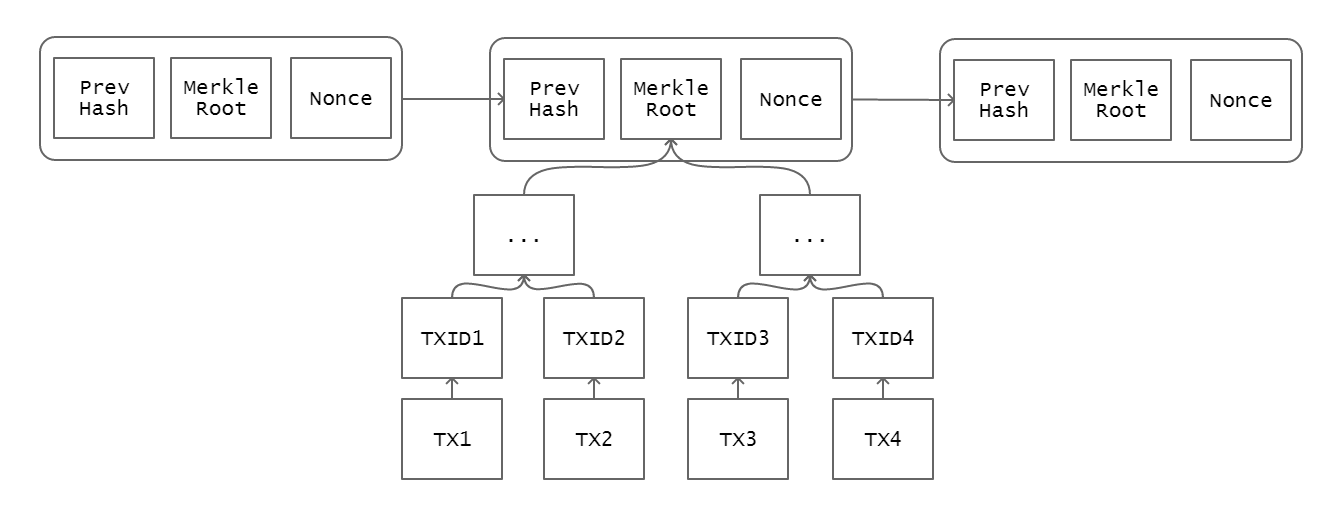
\includegraphics[width=\linewidth]{Images/bitcoin-chain-tx.png}
		\caption[Simplified scheme of the Bitcoin chain]{Simplified scheme of the Bitcoin chain. The block header is richer and the transaction Merkle tree can be deeper}
		\label{fig:tx-chain}
	\end{center}
\end{figure}

The first block, called \textit{genesis block}, cannot include a previous timestamp, the field is set to $\{0\}^{256}$. The block include in the coinbase transaction the headline of The Times:
\begin{quotation}
\textquotedblleft The Times 03/Jan/2009 Chancellor on brink of second bailout for banks\textquotedblright 
\end{quotation}
It proves that the hash was computed after that newspaper was distributed. 
Since each block is a commitment of the previous block, every block is a commitment to the headline inserted by Nakamoto.

Every bitcoin owner \textit{without trusting other users} can broadcast \textit{without any permission} a transaction to the network, a miner will include it in a new block which is appended to the chain or, in other words, it will be timestamped. Every network full node stores an entire copy of the chain to ensure the correctness of all bitcoin transactions ever made, thus the timestamp attestations are \textit{widely published}.  

Assuming the majority of the nodes does not collaborate to attack the network, the cost of rewriting past blocks in the chain grows exponentially, making de facto impossible to change the chain. For this reason, provided not considering the very last blocks, the chain is said to be \textit{immutable}. 

Thus the Bitcoin network is a decentralized, trustless, permissionless notary. Its attestations are stored in a widely published and immutable timestamps chain, which defines the network (and vice versa). 

Bitcoin does something more than timestamping, Nakamoto consensus ensures that each UTXO is spent only once, thus to publish a transaction on the chain is necessary to follow the consensus rules. 
Anyway while playing in the consensus framework it's still possible to write arbitrary data inside a transaction.
As a premise note that a valid transaction can be mined, but not all valid transactions are relayed by nodes, indeed to strengthen the network and the resilience of nodes only \textit{standard} transactions are relayed. This is a common practice between nodes, not a consensus rule, it may be changed if new useful transaction types are proposed. By the time of writing the standard transactions are:
\begin{itemize}
	\item Pay-to-Public-Key (P2PK)
	\item Pay-to-Public-Key-Hash (P2PKH)
	\item Pay-to-Script-Hash (P2SH)
	\item Multisig
	\item Null Data (OP\_RETURN)
\end{itemize}

In the following sections we show two ways to timestamp arbitrary data $d$ into the chain; the idea behind those is summarized in Figure \ref{fig:chain-data}.

\begin{figure}
	\begin{center}
		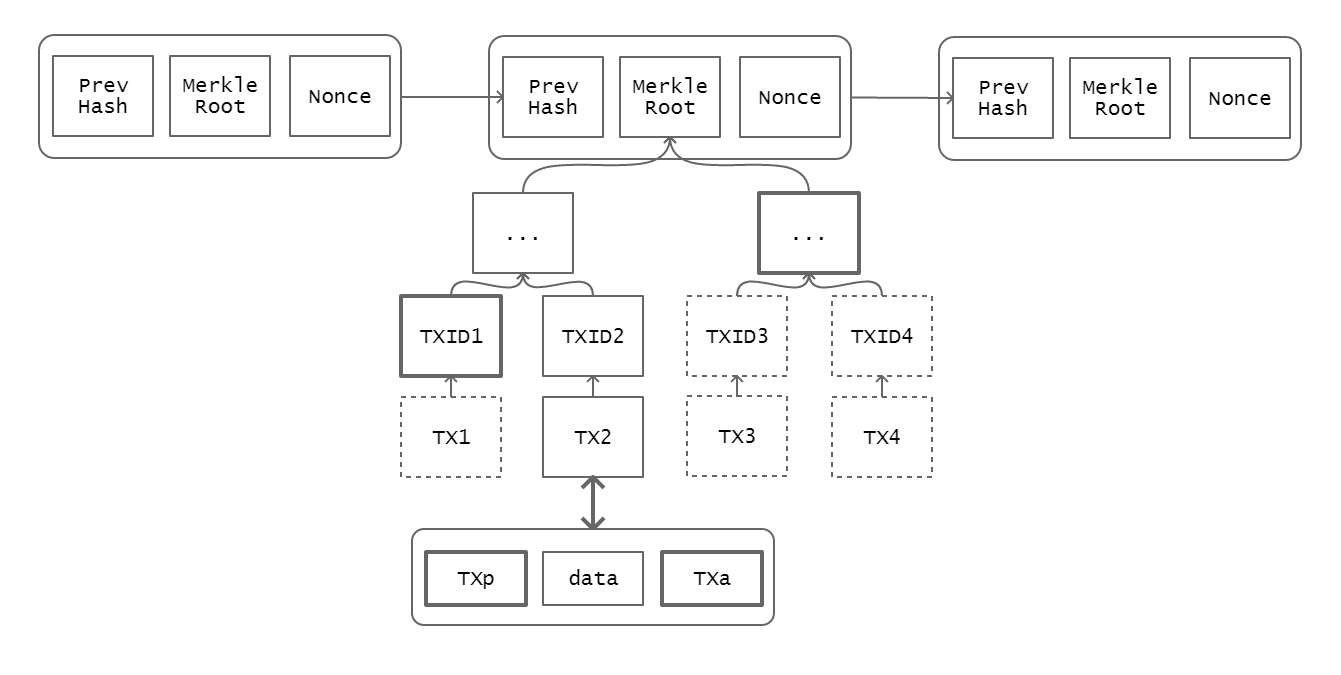
\includegraphics[width=\linewidth]{Images/bitcoin-chain-data-path.png}
		\caption[Commit arbitrary data in the Bitcoin chain]{Commit arbitrary data in the Bitcoin chain. The transaction $TX_2$ includes some data, in the sense that $TX_2=TX_p||data||TX_a$.}
		\label{fig:chain-data}
	\end{center}
\end{figure}

\section{Address Commitment}
Consider the case of a transaction with one P2PKH output. In theory the output contains the hash value of the receiver public key computed applying SHA256 and then RIPEMD160, such value is called \textit{address}. The locking puzzle or \textit{pubkey script} is:
\begin{verbatim}
OP_DUP OP_HASH160 <PubKeyHash> OP_EQUALVERIFY OP_CHECKSIG
\end{verbatim}
The receiver, who knows the corresponding private key can redeem the bitcoin locked with an unlocking script or \textit{signature script} of this kind:
\begin{verbatim}
<sig> <pubkey>
\end{verbatim} 
To provide a timestamp for the data $d$ it is possible to compute the RIPEMD160 hash of $d$ and put it in place of the public key hash:
\begin{verbatim}
OP_DUP OP_HASH160 <DataHash> OP_EQUALVERIFY OP_CHECKSIG
\end{verbatim}
However this pubkey script is not redeemable (unless $d$ is a public key with known private key). Hence the bitcoin associated to this UTXO are lost, but a commitment to $d$ will be timestamped in the chain. 
This technique can also be used to prove that some bitcoin have been destroyed, called \textit{proof-of-burn}.

Even though is a viable and working solution this technique should be avoided, the burned output will stay forever in the database of the UTXO stored by every full node, called \textit{mempool}. If this happens consistently, it will bloat the mempool, adding an additional burden in running a full node, which is not good for the decentralization of the network.

% script op code
\section{OP\_RETURN}
To mitigate the UTXO bloat problem, with the Bitcoin Core 0.9.0 release, a new script opcode, OP\_RETURN, was introduced. An OP\_RETURN change creates a \textit{provably-prunable} output, with script pubkey:
\begin{verbatim}
OP_RETURN <Data>
\end{verbatim}
Such output is provably unspendable, thus it will probably have zero bitcoin locked in, unless used for proof-of-burn. The data field can be filled with at most 80 bytes of arbitrary data. 

OP\_RETURN is used for different purposes, writing raw data on the chain, adding information related to assets linked to a coin or timestamping. Sometimes the data field starts with a prefix indicating if a second layer protocol is being used \cite{DBLP:conf/fc/BartolettiP17}. 

To create a timestamp for some data $d$ with arbitrary size one should add to his transaction an OP\_RETURN change followed by the hash value of $d$ with zero bitcoin associated. If the hash function used has a 32 bytes output, this increases the size of his transaction by 43 bytes (amount 8 bytes, length script pubkey 1 byte, OP\_RETURN 1 byte, length data field 1 byte, data 32 bytes) leading to a lower fee (measured in sat/byte\footnote{After segwit the correct metric to use is sat/vbyte instead of sat/byte}.) which may slow down confirmation time or may lead the user to increase the overall fee, thus including an OP\_RETURN \textit{has a cost}.

In addition it is important to point out that when one wants to timestamp he has also to perform a bitcoin transaction. It may be a transaction that he would have done anyway, but in case these two needs do not coincide, he has to send some bitcoins to himself adding the OP\_RETURN change to actually write something on the chain.
Moreover transactions including OP\_RETURN are easy to spot, hence malicious miners may decide to censor those. A solution is using address commitment, which can be censored only by censoring all the UTXO spendable by all the users who want to timestamp data, which is extremely hard.
Keeping this in mind, if there is no fear of censorship, which presumably happens in most cases, then OP\_RETURN is the correct tool for timestamping.